\documentclass{article}
\usepackage[margin=1in]{geometry}
\usepackage{graphicx}
\usepackage[colorlinks=true, urlcolor=blue]{hyperref}
\usepackage{multicol}
\usepackage{mathpazo}
\usepackage{fancyvrb}

\def\lsmversion{1.10} %%% UPDATE THIS!

\title{Using the \texttt{lsmeans} Package}
\author{Russell V. Lenth\\The University of Iowa\\ 
\texttt{\href{mailto:russell-lenth@uiowa.edu}{russell-lenth@uiowa.edu}}}
\date{Updated with \code{lsmeans} Version~\lsmversion---\today}
%\VignetteIndexEntry{Using the lsmeans package}
%\VignetteDepends{lsmeans}
%\VignetteKeywords{least-squares means}
%\VignettePackage{lsmeans}


\DefineShortVerb{\"}
\DefineVerbatimEnvironment{Winput}{Verbatim}{fontshape=sl}
\DefineVerbatimEnvironment{Woutput}{Verbatim}{}
\def\bottomfraction{.5}
%\def\botfigrule{\hrule}
%\def\topfigrule{\hrule}
\def\code{\texttt}




%%% NOTE This document is actually the .tex file generated by StatWeave %%%
%%%\usepackage{Statweave} %%% Needed stuff is already in preamble
\usepackage{Sweave}
\begin{document}
\maketitle{}

\section{What are least-squares means?}
\subsection{Introduction}
Least-squares means (or LS means), are generalizations of covariate-adjusted means, and date back at least to 1976 when they were incorporated in the contributed SAS procedure named \code{HARVEY} (Harvey 1976). Later, they were incorporated via \code{LSMEANS} statements in the regular SAS releases. SAS's documentation describes them as ``predicted population margins---that is, they estimate the marginal means over a balanced population'' (SAS Institute 2012).

People disagree on the appropriateness of LS~means. As in many statistical calculations, there are times when they are, and times when they are not. However, if one understands what is being calculated, one can judge its appropriateness. So the first task is to try to explain LS~means as clearly as possible. To that end, I offer this:
\begin{quote}\it
LS means are predictions from a model over a grid of predictor values; or marginal averages thereof. 
\end{quote}
More explicitly, define a set of \emph{reference levels}\footnote{I made up this term for convenience in explaining this stuff.} for each predictor, and create a grid consisting of all combinations of these. Make predictions on this grid, and (as needed), compute marginal means of those predictions, usually using equal weights.

The default in the "lsmeans" function is to set the reference levels as follows:
\begin{description}
\item[Factors] For predictors of class "factor" or "ordered", the default reference levels are the levels of the factor.
\item[Covariates] For numeric predictors, the default is to use a single reference level at the mean value of the predictor.
\end{description}

\subsection{Illustration}
To illustrate, consider the randomized block experiment given as an example in Box \emph{et al.} (2005), Table~4.4, page~146. In this experiment on penicillin manufacturing, five blocks (blends of material) were each tested with four treatments (variants of the process), and the process yield is measured.

To save space, I'll use just the data from the first three blends; and to make the example more interesting, suppose that a couple of the observations got lost. Let's enter the data and fit a model:
\begin{Winput}
R> penicillin = expand.grid(treat = LETTERS[1:4], blend = factor(1:3))
R> penicillin$yield = c (
R>     89, 88, 97, 94,
R>     84, 77, NA, 79,
R>     NA, 87, 87, 85
R> )
R> penicillin.lm = lm(yield ~ treat + blend, data = penicillin)
\end{Winput}
The reference levels are simply the factor levels.
Here are the LS~means for the factor combinations (as specified by "~ treat * blend" in the call):
\begin{Winput}
R> library(lsmeans)
R> lsmeans(penicillin.lm, ~ treat * blend)
\end{Winput}
\begin{multicols}{2}\small
\begin{Woutput}
$`treat:blend lsmeans`
 treat blend lsmean     SE df lower.CL upper.CL
     A     1 92.029 2.8970  4   83.985  100.072
     B     1 89.571 2.5865  4   82.390   96.753
     C     1 94.829 2.8970  4   86.785  102.872
     D     1 91.571 2.5865  4   84.390   98.753
     A     2 80.971 2.8970  4   72.928   89.015
     B     2 78.514 2.7239  4   70.952   86.077
     C     2 83.771 3.6744  4   73.570   93.973
     D     2 80.514 2.7239  4   72.952   88.077
     A     3 86.371 3.6744  4   76.170   96.573
     B     3 83.914 2.7239  4   76.352   91.477
     C     3 89.171 2.8970  4   81.128   97.215
     D     3 85.914 2.7239  4   78.352   93.477
\end{Woutput}

\end{multicols}

One can verify that these are simply the predicted values from the model for all 12 factor combinations (including those where there are missing values):
\begin{Winput}
R> predict(penicillin.lm, newdata = penicillin)
\end{Winput}
\begin{Woutput}
     1      2      3      4      5      6      7      8      9     10     11     12
92.029 89.571 94.829 91.571 80.971 78.514 83.771 80.514 86.371 83.914 89.171 85.914
\end{Woutput}
The LS~means for "treat" are simply the marginal averages of these values over the five blends:
\begin{Winput}
R> lsmeans(penicillin.lm, ~ treat)
\end{Winput}
\begin{Woutput}
$`treat lsmeans`
 treat lsmean     SE df lower.CL upper.CL
     A 86.457 2.6789  4   79.019   93.895
     B 84.000 2.0633  4   78.271   89.729
     C 89.257 2.6789  4   81.819   96.695
     D 86.000 2.0633  4   80.271   91.729
\end{Woutput}
For treatments $B$ and~$D$, these LS~means are the same as the marginal means of the data; but for treatments $A$ and~$C$, where missing values occur, they are not the data means, but instead they are model-based predictions of those marginal means. This is an example where I believe most would think these LS~means are a reasonable way to summarize the model results.




\section{Analysis-of-covariance example}
Oehlert (2000), p.456 gives a dataset concerning repetitive-motion pain due to typing on three types of ergonomic keyboards. Twelve subjects having repetitive-motion disorders were randomized to the keyboard types, and reported the severity of their pain on a subjective scale of 0--100 after two weeks of using the keyboard. We also recorded the time spent typing, in hours. Here we enter the data, and obtain the plot shown in Figure~\ref{typing-fig}.
\begin{Winput}
R> typing = data.frame(
R>   type = rep(c("A","B","C"), each=4),
R>   hours = c(60,72,61,50, 54,68,66,59, 56,56,55,51),
R>   pain =  c(85,95,69,58, 41,74,71,52, 41,34,50,40))
R> library(lattice)
R> xyplot(pain ~ hours | type, data = typing, layout = c(3,1))
\end{Winput}
\begin{figure}
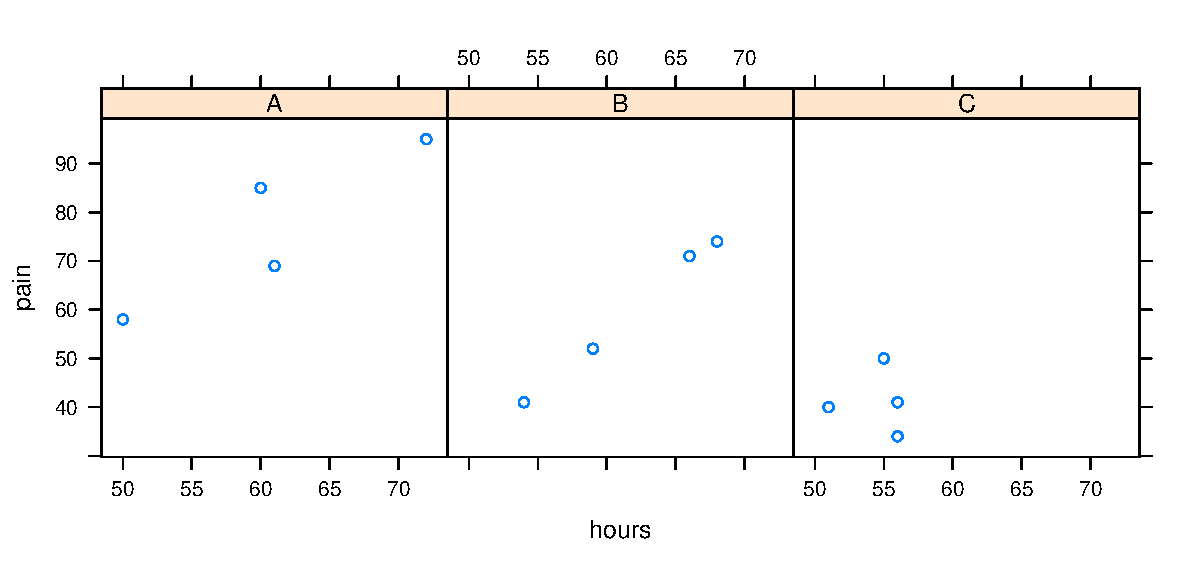
\includegraphics[scale=.75]{using-lsmeans-typing-scatter-fig.pdf}

\caption{Display of the keyboard-pain data.}\label{typing-fig}
\end{figure}


It appears that "hours" and "pain" are linearly related (though it's hard to know for type~$C$ keyboards), and that the trend line for type~$A$ is higher than for the other two. To test this,  consider a simple covariate model that fits parallel lines to the three panels:
\begin{Winput}
R> typing.lm = lm(pain ~ hours + type, data = typing)
\end{Winput}
As mentioned above, the reference levels for "type" are the three keyboard types, whereas the reference levels for "hours" is the mean value of "hours" over the whole dataset:
\begin{Winput}
R> lsmeans(typing.lm, list(~ type, ~ type * hours))
\end{Winput}
\begin{multicols}{2}\small
\begin{Woutput}
$`type lsmeans`
 type lsmean     SE df lower.CL upper.CL
    A 73.565 3.6406  8   65.170   81.960
    B 54.495 3.7223  8   45.912   63.079
    C 49.440 3.9434  8   40.346   58.533

$`type:hours lsmeans`
 type hours lsmean     SE df lower.CL upper.CL
    A    59 73.565 3.6406  8   65.170   81.960
    B    59 54.495 3.7223  8   45.912   63.079
    C    59 49.440 3.9434  8   40.346   58.533
\end{Woutput}

\end{multicols}
The second table shows explicitly that only one reference value is used for the covariate, "hours", hence each table has the same LS~means. These results are the same as what are often called ``adjusted means'' in the analysis of covariance---predicted values for each keyboard type, when the covariate is set to its overall average value.

We can use the "at" argument to override the default reference grid. For example, suppose we want to consider "hours" values of $(55,59,64)$:
\begin{Winput}
R> lsmeans(typing.lm, list(~ type * hours, ~ type, ~ hours),
R>     at = list(hours = c(55,59,64)))
\end{Winput}
\begin{Woutput}
$`type:hours lsmeans`
 type hours lsmean     SE df lower.CL upper.CL
    A    55 66.286 4.1548  8   56.705   75.867
    B    55 47.216 4.3512  8   37.182   57.250
    C    55 42.160 3.5886  8   33.885   50.435
    A    59 73.565 3.6406  8   65.170   81.960
    B    59 54.495 3.7223  8   45.912   63.079
    C    59 49.440 3.9434  8   40.346   58.533
    A    64 82.665 3.7757  8   73.958   91.371
    B    64 63.595 3.6771  8   55.115   72.074
    C    64 58.539 4.9904  8   47.031   70.047

$`type lsmeans`
 type lsmean     SE df lower.CL upper.CL
    A 74.172 3.6212  8   65.821   82.522
    B 55.102 3.6912  8   46.590   63.614
    C 50.046 3.9958  8   40.832   59.260

$`hours lsmeans`
 hours lsmean     SE df lower.CL upper.CL
    55 51.887 2.5337  8   46.044   57.730
    59 59.167 2.0692  8   54.395   63.938
    64 68.266 2.7608  8   61.900   74.633
\end{Woutput}
The first set of LS~means are the same as before when "hours" equals 59. But the marginal LS~means for "type" are different from those before because we have averaged over the predictions for three different "hours" values. This is an example where the marginal LS~means for "type" probably \emph{don't} make a lot of sense, unless there is a really good reason for picking those three particular "hours" values. On the other hand, the LS~means for "hours" do make sense, as they represent the average of the predictions for all three keyboard types.


\section{Contrasts and comparisons}
Often, we want to perform multiple comparisons or contrasts among a set of LS~means. "lsmeans" provides for this by specifying something on the left-hand side of the formula. For example, in the keyboard-pain example, we can obtain pairwise comparisons among the adjusted means as follows:
\begin{Winput}
R> lsmeans(typing.lm, pairwise ~ type)
\end{Winput}
\begin{Woutput}
$`type lsmeans`
 type lsmean     SE df lower.CL upper.CL
    A 73.565 3.6406  8   65.170   81.960
    B 54.495 3.7223  8   45.912   63.079
    C 49.440 3.9434  8   40.346   58.533

$`type pairwise differences`
      estimate     SE df t.ratio p.value
A - B  19.0699 5.0816  8 3.75272 0.01378
A - C  24.1257 5.5596  8 4.33947 0.00621
B - C   5.0558 5.7195  8 0.88395 0.66470
    p values are adjusted using the tukey method for 3 means
\end{Woutput}
Note that "lsmeans" produces two tables for ach two-sided formula---the first is the LS~means, and the second is the contrast output. 

There are other choices besides "pairwise". The other built-in options are "revpairwise" (same as "pairwise" but the subtraction is done the other way; "trt.vs.ctrl" for comparing one factor level (say, a control) with each of the others, and the related "trt.vs.ctrl1", and "trt.vs.ctrlk" for convenience in specifying which group is the control group; "poly" for estimating orthogonal-polynomial contrasts, assuming equal spacing; and "effects" and "del.effects", which compare each LS~mean with the average of all (or all others). It is possible to provide custom contrasts as well---see the documentation.

As seen in the previous output, "lsmeans" provides for adjusting the $p$~values of contrasts to preserve a familywise error rate. The default for pairwise comparisons is the Tukey (HSD) method. One must use these adjustments with caution. For example, when the standard errors are unequal, the Tukey method is only approximate, even under normality and independence assumptions. 
To get a more exact adjustment, we can pass the comparisons to the "glht" function in the "multcomp" package (and also pass additional arguments---in the coming example, none). Then the returned value for the contrasts is a "glht" object instead of a "data.frame":
\begin{Winput}
R> library(multcomp)
R> typing.lsm = lsmeans(typing.lm, pairwise ~ type, glhargs=list())
R> typing.lsm[[2]]
\end{Winput}
\begin{Woutput}
	 Simultaneous Tests for General Linear Hypotheses

Fit: lm(formula = pain ~ hours + type, data = typing)

Linear Hypotheses:
           Estimate Std. Error t value Pr(>|t|)
A - B == 0    19.07       5.08    3.75   0.0138 *
A - C == 0    24.13       5.56    4.34   0.0061 **
B - C == 0     5.06       5.72    0.88   0.6642
---
Signif. codes:  0 '***' 0.001 '**' 0.01 '*' 0.05 '.' 0.1 ' ' 1
(Adjusted p values reported -- single-step method)
\end{Woutput}
These $p$~values are exact (if the assumptions hold) and, as expected, slightly different from those in the previous "lsmeans" output. We may of course use other methods available for "glht" objects. The plot below displays the comparisons in the preceding tabls:
\begin{Winput}
R> plot(typing.lsm[[2]])
\end{Winput}
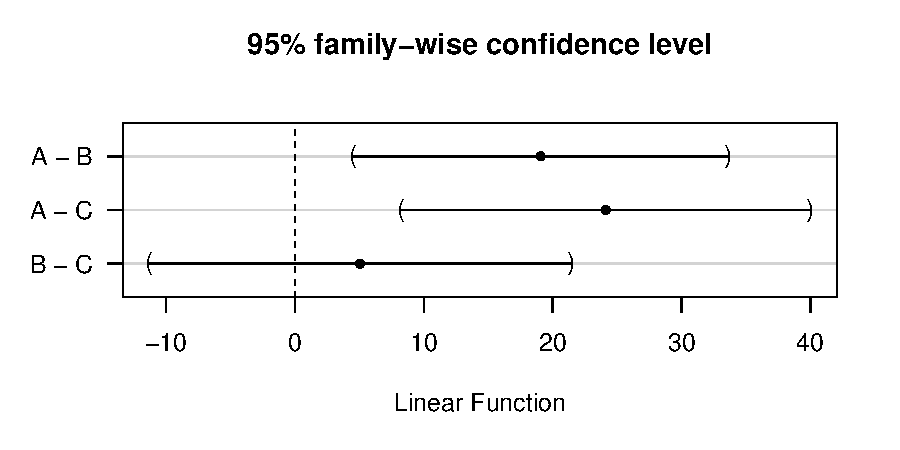
\includegraphics[scale=.6]{using-lsmeans-typing-glht-plot-fig.pdf}

Besides being able to call "glht" from "lsmeans", we have also provided an "lsm" function and an associated "glht" method so that we can call "lsmeans" from within "glht". We use "lsm" in much the same way as "mcp" in the "multcomp" package. Here we display simultaneous confidence intervals for the LS~means:
\begin{Winput}
R> typing.glht = glht(typing.lm, linfct = lsm(~ type))
R> plot(typing.glht)
\end{Winput}
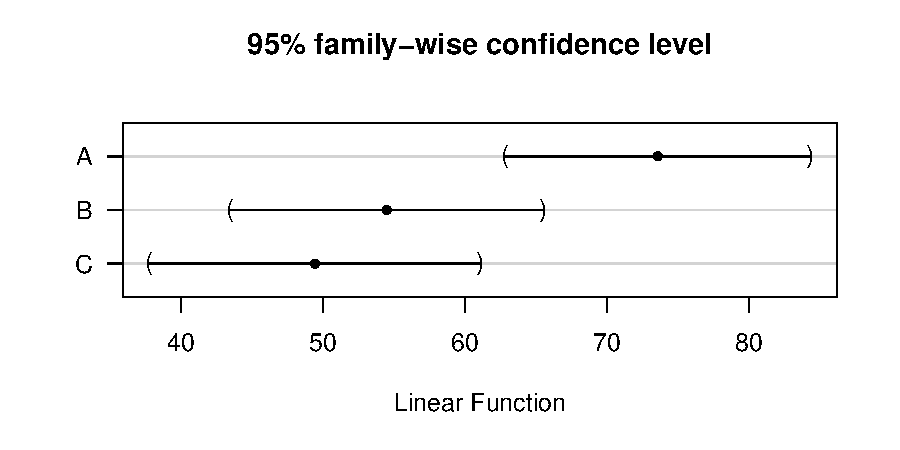
\includegraphics[scale=.6]{using-lsmeans-typing-confint-plot-fig.pdf}
\\
Unlike "lsmeans" which returns a list, the design of "lsm" is to create just one set of linear functions to hand to "glht". It returns contrast output if available, otherwise LS~means output; so In the illustration above, the linear functions of the lsmeans themselves are used. If we had instead specified "lsm(pairwise ~ type)", then the results would have been the same as shown earlier for the pairwise differences. 


\section{Two-factor example}
Now consider the R-provided dataset "warpbreaks", relating to a weaving-process experiment. This dataset (from Tukey 1977, p.82) has two factors: "wool" (two types of wool), and "tension" (low, medium, and high); and the response variable is "breaks", the nuumber of breaks in a fixed length of yarn.
%To make it more interesting, we'll delete some cases so that the design is unbalanced.
% \begin{Rcode}
% warp = warpbreaks[-c(1,2,3,5,8,13,21,34), ]
% with(warp, table(wool, tension))
% \end{Rcode}
\begin{Winput}
R> with(warpbreaks, table(wool, tension))
\end{Winput}
\begin{Woutput}
    tension
wool L M H
   A 9 9 9
   B 9 9 9
\end{Woutput}
Let us fit a model that includes interaction
\begin{Winput}
R> warp.lm = lm(breaks ~ wool * tension, data = warpbreaks)
R> anova(warp.lm)
\end{Winput}
\begin{Woutput}
Analysis of Variance Table

Response: breaks
             Df Sum Sq Mean Sq F value  Pr(>F)
wool          1    451     451    3.77 0.05821 .
tension       2   2034    1017    8.50 0.00069 ***
wool:tension  2   1003     501    4.19 0.02104 *
Residuals    48   5745     120
---
Signif. codes:  0 '***' 0.001 '**' 0.01 '*' 0.05 '.' 0.1 ' ' 1
\end{Woutput}
The "lsmeans" package provides a function "lsmip" that provides an interaction plot based on the LS~means:
\begin{Winput}
R> lsmip(warp.lm, wool ~ tension)
\end{Winput}
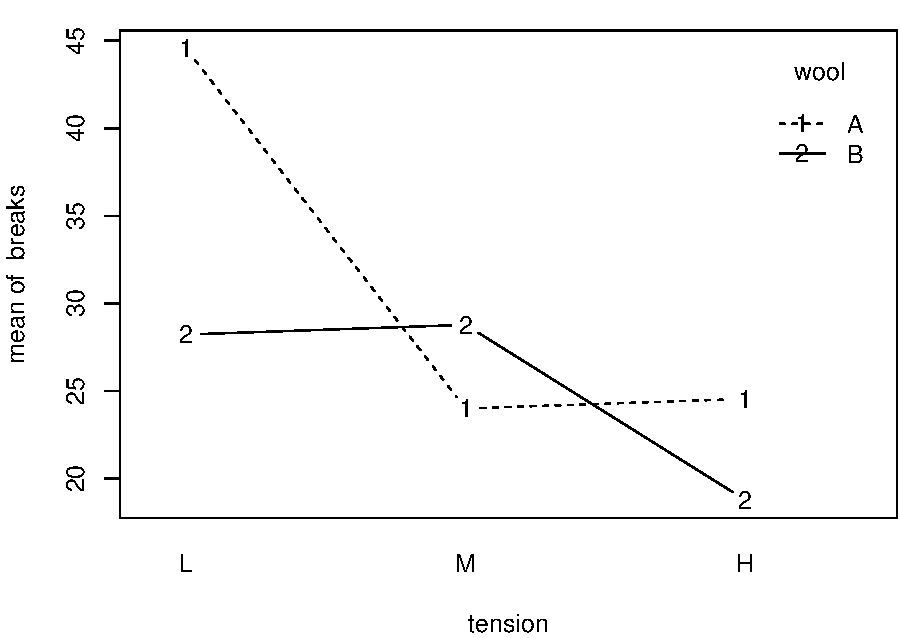
\includegraphics[scale=.5]{using-lsmeans-warp-intplot-fig.pdf}
\\
Now we can obtain the least-squares means for the "wool"$\times$"tension" combinations. We could request pairwise comparisons as well by specifying "pairwise ~ wool:tension", but this will yield quite a few comparisons (15 to be exact). Often, people are satisfied with a smaller number of comparisons (or contrasts) obtained by restricting them to be at the same level of one of the factors. This can be done using the "|" symbol for conditioning. In the code below, we request comparisons of the wools at each tension, and polynomial contrasts for each wool.
\begin{Winput}
R> print(lsmeans(warp.lm, list(pairwise ~ wool | tension,  poly ~ tension | wool)), omit=3)
\end{Winput}
\begin{Woutput}
$`wool:tension lsmeans`
 wool tension lsmean     SE df lower.CL upper.CL
    A       L 44.556 3.6468 48   37.223   51.888
    B       L 28.222 3.6468 48   20.890   35.555
    A       M 24.000 3.6468 48   16.668   31.332
    B       M 28.778 3.6468 48   21.445   36.110
    A       H 24.556 3.6468 48   17.223   31.888
    B       H 18.778 3.6468 48   11.445   26.110

$`wool:tension pairwise differences`
          estimate     SE df  t.ratio p.value
A - B | L  16.3333 5.1573 48  3.16703 0.00268
A - B | M  -4.7778 5.1573 48 -0.92641 0.35887
A - B | H   5.7778 5.1573 48  1.12031 0.26816
    p values are adjusted using the tukey method for 2 means

$`tension:wool polynomial contrasts`
              estimate     SE df t.ratio p.value
linear | A    -20.0000 5.1573 48 -3.8780 0.00032
quadratic | A  21.1111 8.9327 48  2.3634 0.02221
linear | B     -9.4444 5.1573 48 -1.8313 0.07327
quadratic | B -10.5556 8.9327 48 -1.1817 0.24315
    p values are not adjusted
\end{Woutput}
(We suppressed the third element of the results because it is the same as the first, with rows rearranged.)
With these data, the least-squares means are exactly equal to the cell means of the data.
The main result (visually clear in the interaction plot) is that the wools differ the most when the tension is low. The signs of the polynomial contrasts indicate decrasing trends for both wools, but opposite concavities.

It is also possible to abuse "lsmeans" with a call like this:
\begin{Winput}
R> lsmeans(warp.lm, ~ wool)   ### NOT a good idea!
\end{Winput}
\begin{Woutput}
$`wool lsmeans`
 wool lsmean     SE df lower.CL upper.CL
    A 31.037 2.1055 48   26.804   35.270
    B 25.259 2.1055 48   21.026   29.493

Warning message:
In lsmeans(warp.lm, ~wool) :
  lsmeans of wool may be misleading due to interaction with other predictor(s)
\end{Woutput}
Each lsmean is the average of the three "tension" lsmeans at the given "wool". As the warning indicates, the presence of the strong interaction indicates that these results are pretty meaningless. In another dataset where an additive model would explain the data, these marginal averages, and comparisons or contrasts thereof, can nicely summarize the main effects in an interpretable way.

\section{Split-plot example}
The "nlme" package includes a famous dataset "Oats" that was used in Yates~(1935) as an example of a split-plot experiment. Here is a summary of the dataset.
\begin{Winput}
R> data(Oats, package="nlme")
R> summary(Oats)
\end{Winput}
\begin{Woutput}
 Block           Variety       nitro          yield
 VI :12   Golden Rain:24   Min.   :0.00   Min.   : 53
 V  :12   Marvellous :24   1st Qu.:0.15   1st Qu.: 86
 III:12   Victory    :24   Median :0.30   Median :102
 IV :12                    Mean   :0.30   Mean   :104
 II :12                    3rd Qu.:0.45   3rd Qu.:121
 I  :12                    Max.   :0.60   Max.   :174
\end{Woutput}
The experiment was conducted in six blocks, and each block was divided into three plots, which were randomly assigned to varieties of oats. With just "Variety" as a factor, it is a randomized complete-block experiment. However, each plot was subdivided into 4 subplots and the subplots were treated with different amounts of nitrogen. Thus, "Block" is a blocking factor, "Variety" is the whole-plot factor, and "nitro" is the split-plot factor. The response variable is "yield", the yield of each subplot in bushels per~acre. Below is an interaction plot of these data.
\begin{Winput}
R> with(Oats, interaction.plot(nitro, Variety, yield, type="b"))
\end{Winput}
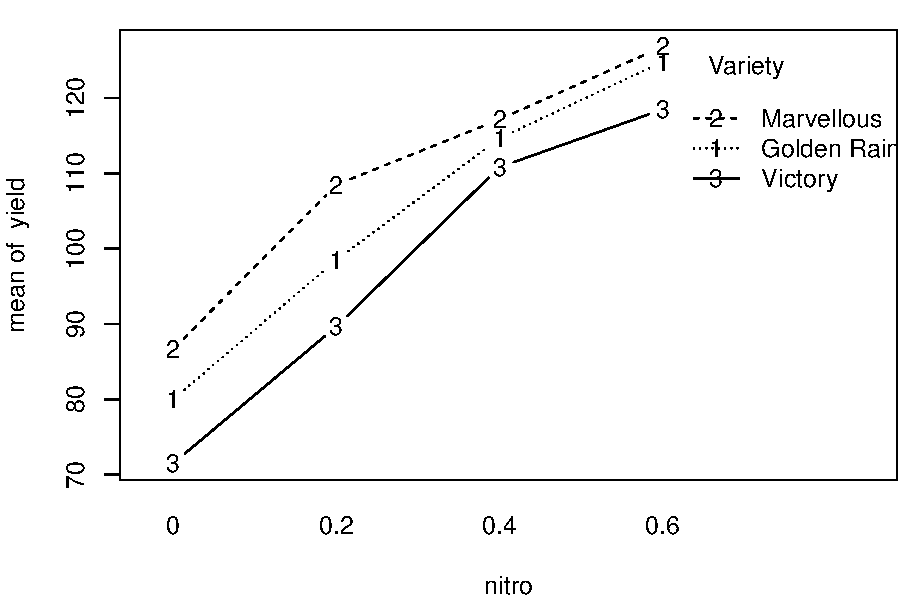
\includegraphics[scale=.5]{using-lsmeans-oats-intplot-fig.pdf}
%\hfill
%\begin{Rcode}{fig, !echo, hide, scale=.5, height=4, label=oats-intplot2}
%par(mar=c(4,4,1,.1))
%library(lme4)
%Oats.lmer = lmer(yield ~ Variety + factor(nitro) + (1 | Block/Variety), data=Oats)
%Oats.lsms = lsmeans(Oats.lmer, ~ nitro:Variety)
%with(Oats.lsms[[1]], interaction.plot(nitro, Variety, lsmean, type="b", ylab="Least-Squares means"))
%\end{Rcode}
\\
There is not much evidence of an interaction. In this dataset, we have random factors "Block" and "Block:Variety" (which identifies the plots). So we will fit a linear mixed-effects model that accounts for these. Another technicality is that "nitro" is a numeric variable, and initially we will model it as a factor. We will use "lmer" in the "lme4" package to fit a model, and display the marginal LS~means with appropriate contrasts.
\enlargethispage{-36pt} %%% MANUAL FORMATTING %%%
\begin{Winput}
R> library(lme4)
R> Oats.lmer = lmer(yield ~ Variety + factor(nitro) + (1 | Block/Variety), data=Oats)
R> lsmeans(Oats.lmer, list(revpairwise ~ Variety,  poly ~ nitro))
\end{Winput}
\begin{Woutput}
Loading required package: pbkrtest
Loading required package: MASS
Loading required package: parallel
$`Variety lsmeans`
     Variety  lsmean     SE    df lower.CL upper.CL
 Golden Rain 104.500 7.7975 8.869   86.821   122.18
  Marvellous 109.792 7.7975 8.869   92.113   127.47
     Victory  97.625 7.7975 8.869   79.946   115.30

$`Variety pairwise differences`
                         estimate     SE df  t.ratio p.value
Marvellous - Golden Rain   5.2917 7.0789 10  0.74753 0.74187
Victory - Golden Rain     -6.8750 7.0789 10 -0.97120 0.61035
Victory - Marvellous     -12.1667 7.0789 10 -1.71873 0.24583
    p values are adjusted using the tukey method for 3 means

$`nitro lsmeans`
 nitro  lsmean     SE     df lower.CL upper.CL
   0.0  79.389 7.1324 6.6386   62.336   96.442
   0.2  98.889 7.1324 6.6386   81.836  115.942
   0.4 114.222 7.1324 6.6386   97.169  131.276
   0.6 123.389 7.1324 6.6386  106.336  140.442

$`nitro polynomial contrasts`
          estimate      SE df  t.ratio p.value
linear     147.333 13.4395 51 10.96268 0.00000
quadratic  -10.333  6.0103 51 -1.71926 0.09163
cubic       -2.000 13.4395 51 -0.14881 0.88229
    p values are not adjusted
\end{Woutput}
The polynomial contrasts for "nitro" suggest that we could substitute a quadratic trend for "nitro"; and if we do that, then there is another (probably better) way to make the above predictions:
\begin{Winput}
R> OatsPoly.lmer = lmer(yield ~ Variety + poly(nitro, 2) + (1 | Block/Variety), data=Oats)
\end{Winput}
The graphs below show the LS~means from these two models.
\begin{multicols}{2}
\begin{Winput}
R> lsmip(Oats.lmer, Variety ~ nitro)
\end{Winput}
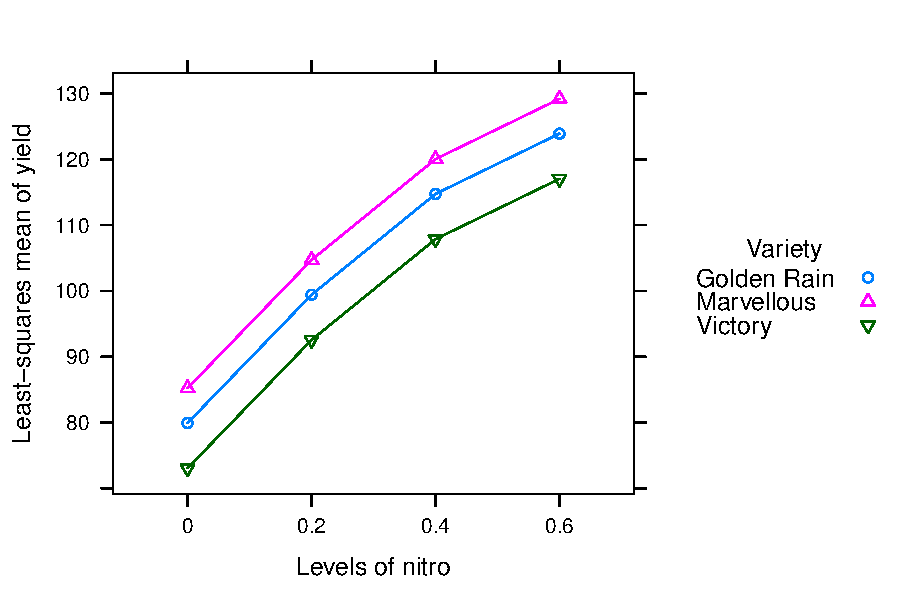
\includegraphics[scale=.5]{using-lsmeans-oat-add-lsmip-fig.pdf}
\begin{Winput}
R> lsmip(OatsPoly.lmer, Variety ~ nitro, 
R>     cov.reduce = FALSE)
\end{Winput}
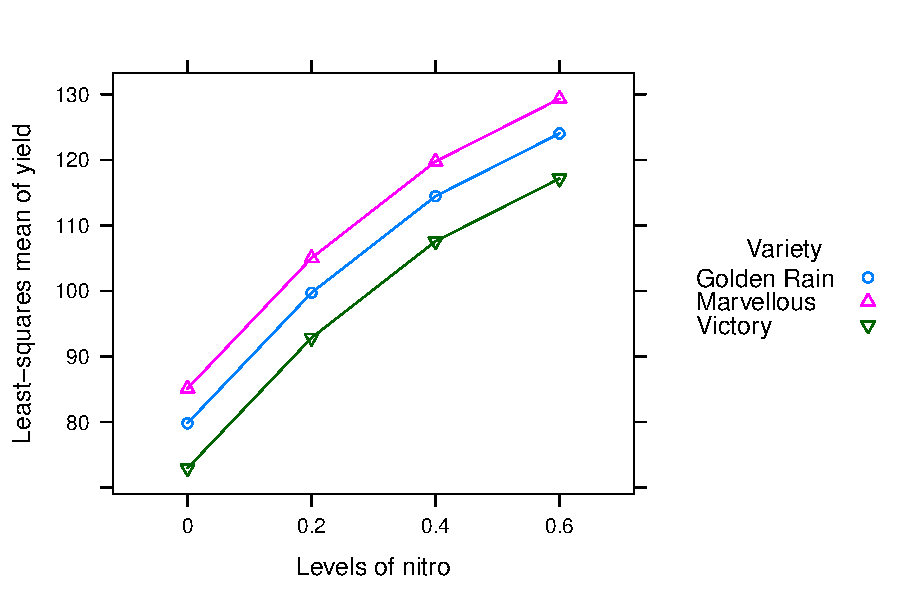
\includegraphics[scale=.5]{using-lsmeans-oat-poly-lsmip-fig.pdf}
\end{multicols}
\noindent
These plots are nearly identical. The "lsmip" function works by calling "lsmeans" with a specification for the required factor combinations. In the second plot, we passed the extra argument "cov.reduce = FALSE" to "lsmeans", which causes it to use the unique values of "nitro" rather than predicting at the average of "nitro".



\section{Messy data}
To illustrate some more issues, and related \code{lsmeans} capabilities, consider the dataset named \code{nutrition} that is provided with the \code{lsmeans} package. These data come from Milliken and Johnson (1984), and contain the results of an observational study on nutrition education. Low-income mothers are classified by race, age category, and whether or not they received food stamps (the \code{group} factor); and the response variable is a gain score (post minus pre scores) after completing a nutrition training program. The graph below displays the data.
\begin{Winput}
R> xyplot(gain ~ age | race*group, data=nutrition)
\end{Winput}
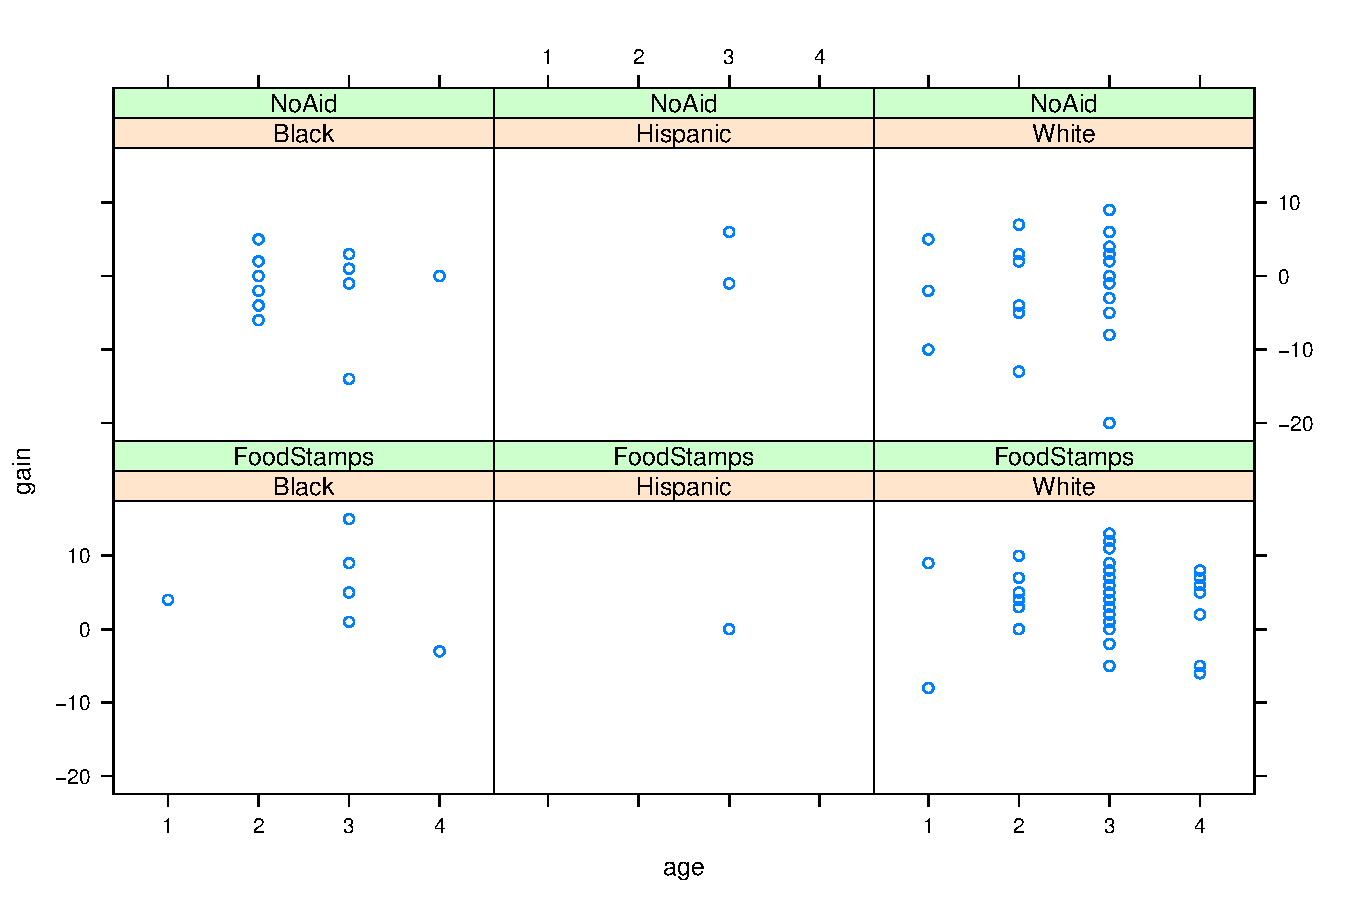
\includegraphics[scale=.5]{using-lsmeans-nutr-scatter-fig.pdf}

Consider the model that includes all main effects and two-way interactions; and let us look at the \code{group} by \code{race} lsmeans:
\begin{Winput}
R> nutr.lm = lm(gain ~ (age + group + race)^2, data = nutrition)
R> lsmeans(nutr.lm, ~ group*race)
\end{Winput}
\begin{Woutput}
$`group:race lsmeans`
      group     race  lsmean     SE df   lower.CL upper.CL
 FoodStamps    Black  4.7083 2.3681 92  0.0049714   9.4115
      NoAid    Black -2.1904 2.4906 92 -7.1368981   2.7561
 FoodStamps Hispanic      NA     NA NA         NA       NA
      NoAid Hispanic      NA     NA NA         NA       NA
 FoodStamps    White  3.6077 1.1556 92  1.3125215   5.9028
      NoAid    White  2.2563 2.3893 92 -2.4889667   7.0016
\end{Woutput}
One thing that this illustrates is that \code{lsmeans} incorporates an estimability check, and returns a missing value when a prediction cannot be made uniquely. In this example, we have very few Hispanic mothers in the dataset, resulting in empty cells. This creates a rank deficiency in the fitted model and some predictors are thrown out.

The "lsmip" function can display a three-way interaction plot

\begin{Winput}
R> lsmip(nutr.lm, race ~ age | group)
\end{Winput}
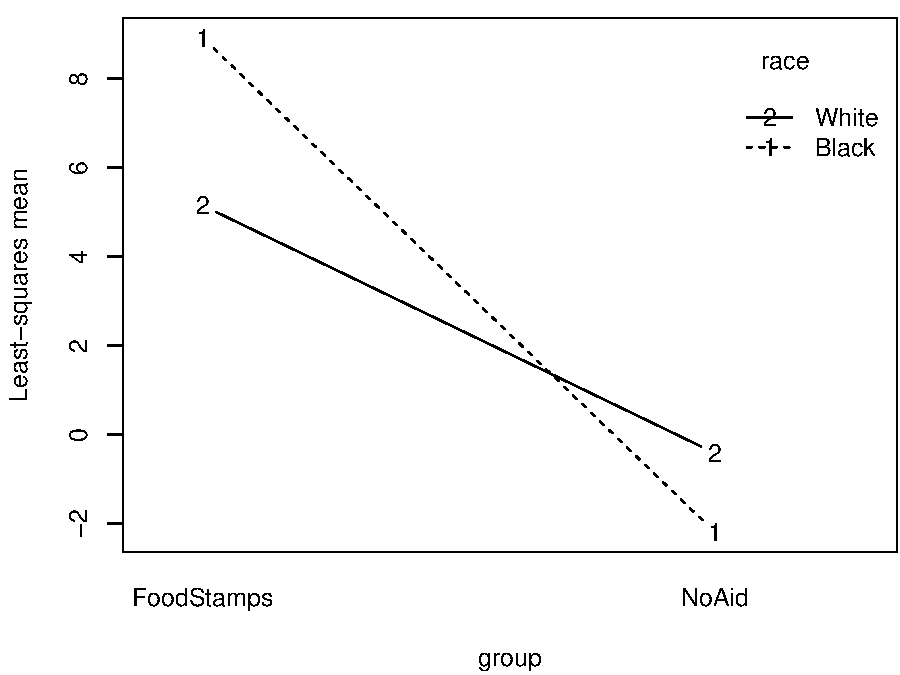
\includegraphics[scale=.75]{using-lsmeans-nutr-intplot-fig.pdf}


We can avoid non-estimable cases by using "at" to restrict the reference levels to a smaller set:
\begin{Winput}
R> lsmeans(nutr.lm, ~ group*race, at = list(age = "3"))
\end{Winput}
\begin{Woutput}
$`group:race lsmeans`
      group     race      lsmean      SE df lower.CL upper.CL
 FoodStamps    Black  7.5000e+00 2.67205 92   2.1931 12.80693
      NoAid    Black -3.6667e+00 2.18172 92  -7.9998  0.66642
 FoodStamps Hispanic  2.1316e-14 5.34411 92 -10.6139 10.61386
      NoAid Hispanic  2.5000e+00 3.77885 92  -5.0051 10.00513
 FoodStamps    White  5.4194e+00 0.95983 92   3.5130  7.32566
      NoAid    White -2.0000e-01 1.19498 92  -2.5733  2.17333
\end{Woutput}
Nonetheless, the standard errors for the Hispanic mothers are enormous due to very small counts.
One useful summary of the results is to narrow the scoe of the reference levels to two races and the two middle age groups, where most of the data lie. Here are the lsmeans and comparisons within rows and columns
\begin{Winput}
R> nutr.lsm = lsmeans(nutr.lm, list(pairwise~group|race, pairwise~race|group),
R>         at = list(age=c("2","3"), race=c("Black","White")))
R> nutr.lsm[-3]
\end{Winput}
\begin{Woutput}
$`group:race lsmeans`
      group  race  lsmean     SE df lower.CL upper.CL
 FoodStamps Black  8.9165 3.4238 92   2.1166 15.71639
      NoAid Black -2.1905 1.4866 92  -5.1430  0.76203
 FoodStamps White  5.1472 1.0596 92   3.0427  7.25168
      NoAid White -0.4125 1.1178 92  -2.6325  1.80755

$`group:race pairwise differences`
                           estimate     SE df t.ratio p.value
FoodStamps - NoAid | Black  11.1070 3.7778 92  2.9400 0.00415
FoodStamps - NoAid | White   5.5597 1.5402 92  3.6097 0.00050
    p values are adjusted using the tukey method for 2 means

$`race:group pairwise differences`
                           estimate     SE df  t.ratio p.value
Black - White | FoodStamps   3.7693 3.3942 92  1.11052 0.26967
Black - White | NoAid       -1.7780 1.8600 92 -0.95592 0.34162
    p values are adjusted using the tukey method for 2 means
\end{Woutput}
The general conclusion from these analyses is that (except for age 4, where the data are very sparse), the expected gains from the training are higher among families receiving food stamps.
Note that this analysis is somewhat different than the results we would obtain by subsetting the data, as we are borrowing information from the other observations in estimating and testing these LS~means.


%\clearpage %-------- MANUAL FORMATTING ---------
\section{GLMM example}
The dataset "cbpp" in the "lme4" package, originally from Lesnoff \emph{et al.}~(1964), provides data on the incidence of contagious bovine pleuropneumonia in 15 herds of zebu cattle in Ethiopia, collected over four time periods. These data are used as the primary example for the "glmer" function, and it is found that a model that accounts for overdisperion is advantageous; hence the addition of the "(1|obs)" in the model fitted below. 

"lsmeans" may be used as in linear models to obtain marginal linear predictions for a generalized linear model or, in this case, a generalized linear mixed model. Here, we use the "trt.vs.ctrl1" contrast family to compare each period with the first, as the primary goal was to track the spread or decline of CBPP over time.
\begin{Winput}
R> cbpp$obs = 1:nrow(cbpp)
R> cbpp.glmer = glmer(cbind(incidence, size - incidence) 
R>    ~ period + (1 | herd) + (1 | obs),  family = binomial,  data = cbpp)
R> anova(cbpp.glmer)   
\end{Winput}
\begin{Woutput}
Analysis of Variance Table
       Df Sum Sq Mean Sq F value
period  3   15.1    5.05    5.05
\end{Woutput}
We will save the results from "lsmean", then add the inverse logits of the predictions and the estimated odds ratios for the comparisons as an aid in interpretation.
\begin{Winput}
R> cbpp.lsm = lsmeans(cbpp.glmer, trt.vs.ctrl1 ~ period)
R> cbpp.lsm[[1]]$pred.incidence = 1 - 1 / (1 + exp(cbpp.lsm[[1]]$lsmean))
R> cbpp.lsm[[2]]$odds.ratio = exp(cbpp.lsm[[2]]$estimate)
R> cbpp.lsm
\end{Winput}
\begin{Woutput}
$`period lsmeans`
 period  lsmean      SE df asymp.LCL asymp.UCL pred.incidence
      1 -1.5003 0.28876 NA   -2.0662  -0.93433       0.182382
      2 -2.7268 0.38097 NA   -3.4735  -1.98010       0.061411
      3 -2.8291 0.39940 NA   -3.6119  -2.04631       0.055771
      4 -3.3665 0.51939 NA   -4.3845  -2.34856       0.033358

$`period differences from control`
      estimate      SE df z.ratio p.value odds.ratio
2 - 1  -1.2265 0.47345 NA -2.5905 0.02851    0.29332
3 - 1  -1.3288 0.48839 NA -2.7208 0.01944    0.26479
4 - 1  -1.8662 0.59056 NA -3.1601 0.00474    0.15470
    p values are adjusted using the sidak method for 3 tests
\end{Woutput}
When degrees of freedom are not available, as in this case, "lsmeans" emphasizes that fact by displaying "NA" for degrees of freedom and in the column headings.
%In a way, the comparisons table is not needed because the results are the same as the regression coefficients under the default parameterization.


\section{Trends}
The "lsmeans" function also provides for estimating and comparing the slopes of fitted lines (or curves). To illustrate, consider the built-in R dataset "ChickWeight" which has data on the growths of newly hatched chicks under four different diets. Here is a display of the dataset.
%The dataset is displayed in Figure~\ref{chick-fig}.
%\begin{figure}
\begin{Winput}
R> xyplot(weight~Time | Diet, groups = ~ Chick, data=ChickWeight, type="o", layout=c(4,1))
\end{Winput}
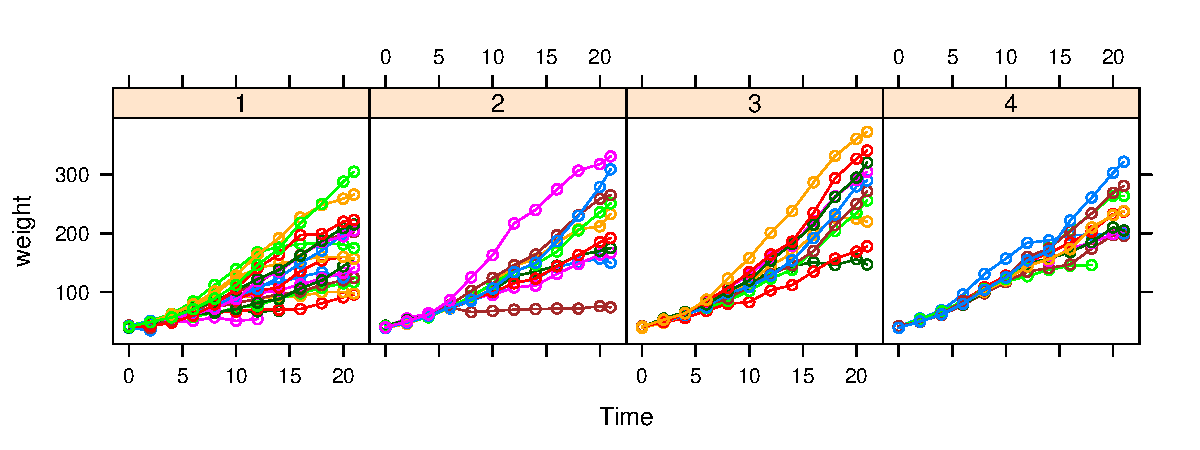
\includegraphics[scale=.8]{using-lsmeans-chick-plot-fig.pdf}
%\caption{Growth curves of chicks, dataset \texttt{ChickWeight}.}\label{chick-fig}
%\end{figure}

Let us fit a model to these data using random slopes for each chick and allowing for a different average slope for each diet:
\begin{Winput}
R> Chick.lmer = lmer(weight ~ Diet * Time + (0 + Time | Chick), data = ChickWeight)
R> print(Chick.lmer, corr = FALSE)
\end{Winput}
\begin{Woutput}
Linear mixed model fit by REML ['lmerMod']
Formula: weight ~ Diet * Time + (0 + Time | Chick)
   Data: ChickWeight

REML criterion at convergence: 4869.6

Random effects:
 Groups   Name Variance Std.Dev.
 Chick    Time   6.67    2.58
 Residual      196.77   14.03
Number of obs: 578, groups: Chick, 50

Fixed effects:
            Estimate Std. Error t value
(Intercept)    33.22       1.77   18.77
Diet2          -4.58       3.00   -1.53
Diet3         -14.97       3.00   -4.98
Diet4          -1.45       3.02   -0.48
Time            6.34       0.61   10.39
Diet2:Time      2.27       1.04    2.19
Diet3:Time      5.08       1.04    4.90
Diet4:Time      3.22       1.04    3.10
\end{Woutput}
Then call "lsmeans" with the "trend" argument to estimate and compare the average slopes for each diet:
\begin{Winput}
R> lsmeans(Chick.lmer, revpairwise ~ Diet, trend = "Time")
\end{Winput}
\begin{Woutput}
$`Time.trend by Diet`
 Diet Time.trend      SE     df lower.CL upper.CL
    1     6.3386 0.61050 49.805   5.1122   7.5649
    2     8.6091 0.83802 48.282   6.9244  10.2938
    3    11.4229 0.83802 48.282   9.7382  13.1076
    4     9.5558 0.83926 48.564   7.8689  11.2428

$`Diet pairwise differences`
      estimate     SE     df  t.ratio p.value
2 - 1  2.27058 1.0368 48.802  2.18995 0.14041
3 - 1  5.08432 1.0368 48.802  4.90376 0.00006
3 - 2  2.81373 1.1851 48.282  2.37417 0.09583
4 - 1  3.21727 1.0378 48.989  3.10002 0.01637
4 - 2  0.94669 1.1860 48.423  0.79821 0.85489
4 - 3 -1.86705 1.1860 48.423 -1.57421 0.40263
    p values are adjusted using the tukey method for 4 means
\end{Woutput}
The tests of comparisons with Diet~1 match those from the regression coefficients, as they should.


\section{Contrasts}
You may occasionally want to know exactly what contrast coefficients are being used, especially in the polynomial case. Contrasts are implemented in functions having names of the form \texttt{\textsl{name}.lsmc} (``lsmc'' for ``least-squares means contrasts''), and you can simply call that function to see the contrasts; for example,
\begin{Winput}
R> poly.lsmc(1:4)
\end{Winput}
\begin{Woutput}
  linear quadratic cubic
1     -3         1    -1
2     -1        -1     3
3      1        -1    -3
4      3         1     1
\end{Woutput}
"poly.lsmc" uses the base function "poly" plus an \emph{ad hoc} algorithm that tries (and usually succeeds) to make integer coefficients, copmparable to what you find in published tables of orthogonal polynomial contrasts.

You may supply your own custom contrasts in two ways. One is to supply a "contr" argument in the "lsmeans" call, like this:
\begin{Winput}
R> print(lsmeans(typing.lm, custom.comp ~ type, 
R>               contr = list(custom.comp = list(fancy.contrast=c(1, -.75, -.25)))), 
R>     omit=1)
\end{Winput}
\begin{Woutput}
$`type custom.comp`
               estimate     SE df t.ratio p.value
fancy.contrast   20.334 4.5783  8  4.4414 0.00216
    p values are not adjusted
\end{Woutput}
Each contrast family is potentially a list of several contrasts, and there are potentially more than one contrast family; so we must provide a list of lists.

The other way is to create your own ".lsmc" function, and use its base name in a formula:
\begin{Winput}
R> inward.lsmc = function(levs, ...) {
R>     n = length(levs)
R>     result = data.frame(`grand mean` = rep(1/n, n))
R>     for (i in 1 : floor(n/2)) {
R>         x = rep(0, n)
R>         x[1:i] = 1/i
R>         x[(n-i+1):n]  = -1/i
R>         result[[paste("first", i, "vs last", i)]] = x
R>     }
R>     attr(result, "desc") = "grand mean and inward contrasts"
R>     attr(result, "adjust") = "none"
R>     result
R> }
\end{Winput}
Testing it, we have
\begin{Winput}
R> inward.lsmc(1:5)
\end{Winput}
\begin{Woutput}
  grand.mean first 1 vs last 1 first 2 vs last 2
1        0.2                 1               0.5
2        0.2                 0               0.5
3        0.2                 0               0.0
4        0.2                 0              -0.5
5        0.2                -1              -0.5
\end{Woutput}
\ldots\ and an application:
\begin{Winput}
R> print(lsmeans(Oats.lmer, inward ~ nitro), omit=1)
\end{Winput}
\begin{Woutput}
$`nitro grand mean and inward contrasts`
                  estimate     SE df  t.ratio p.value
grand.mean         103.972 6.6406  5  15.6570   2e-05
first 1 vs last 1  -44.000 4.2500 51 -10.3530   0e+00
first 2 vs last 2  -29.667 3.0052 51  -9.8719   0e+00
    p values are not adjusted
\end{Woutput}


\section{Differences from SAS}
"lsmeans" started out with a goal of providing similar capabilities to the "LSMEANS" statements in various SAS procedures. The points below do not list all differences from SAS, but may help you understand how they differ and navigate how to translate a SAS specification to an "lsmeans" one.
\begin{itemize}
\item SAS will not print LS~means for factor combinations unless the model contains a corresponding interaction term.
\item SAS allows only factors (i.e., CLASS variables) in the specification of levels for LS~means. The "lsmeans" function allows covariates as well.
\item SAS does not seem to allow multiple "at" values for a covariate.
\item As I understand it, SAS's "OBSMARGINS" ("OM") option allows one to specify a dataset that defines a grid of reference levels. In the R "lsmeans" function, this is done more simply using "at" (or in one special case,  "cov.reduce=FALSE").
\item For unequal weights for the marginal LS~means, in SAS one must construct the "OM" dataset to reflect the desired proportions, or has a "weight" variable; whereas in "lsmeans" we customize the "fac.reduce" function.
\item Some of the capabilities of SAS's "split" and "bylevel" options are provided by using a conditioning symbol ``"|"'' in the "lsmeans" specification to delineate the desired slices. "lsmeans" does not output $F$~tests for the slices.
\end{itemize}

\ifx %-------------------- EXCISED ------------------
In general, now that covariates can be specified in an LS~means specification, the conceptual framework of "lsmeans" has evolved to serve a more general purpose than SAS does of providing predictions for any linear model on a grid of reference levels. For example, suppose that we have a model "mod" that involves a fractor "treat" and a complicated functions of two numeric variables "x1" and "x2". We can use "lsmeans" to easily create the data for side-by-side contour plots of the fitted surface, via code like this:
\begin{Winput}
R> require(lattice)
R> contourplot(lsmean ~ x1*x2|treat, 
R>     data = lsmeans(mod, ~x1*x2|treat, at = list(x1=x1.vals, x2=x2.vals))[[1]])
\end{Winput}
where "x1.vals" and "x2.vals" define the grid of values for the contour plot.
\fi %-------------------- END OF CUT ---------------------

\section*{References}
\begin{description}

\item[Box, G., Hunter,, J., and Hunter, W.~(2005)]
\emph{Statistics for Experimenters} (2nd ed.).
Wiley.

\item[Harvey, W.~(1976)] Use of the HARVEY procedure.
SUGI Proceedings, 
\url{http://www.sascommunity.org/sugi/SUGI76/Sugi-76-20%20Harvey.pdf} (accessed June 20, 2013).

\item[Lesnoff, M., Laval, G., Bonnet, P., \emph{et al.}~(2004)] Within-herd spread of contagious bovine pleuropneumonia in Ethiopian highlands, \emph{Preventive Veterinary Medicine},  \textbf{64}, 27--40.

\item[Milliken, G. A. and Johnson, D. E. (1984)]
\emph{Analysis of Messy Data -- Volume I: Designed Experiments}. Van Nostrand, ISBN 0-534-02713-7.


\item[Oehlert, G. (2000)] \emph{A First Course in Design and Analysis of Experiments}, W.~H.~Freeman.
This is out-of-print, but now available under a Creative Commons license via \url{http://users.stat.umn.edu/~gary/Book.html} (accessed August 23, 2012).

\item[SAS Institute Inc. (2012)]
Online documentation, SAS/STAT version 9.3: Shared concepts: LSMEANS statement.
\url{http://support.sas.com/documentation/cdl/en/statug/63962/HTML/default/viewer.htm#statug_introcom_a0000003362.htm} (accessed August 14, 2012).

\item[Tukey, J.~W.~(1977)] \emph{Exploratory Data Analysis}. Addison-Wesley. 

\item[Yates, F. (1935)] Complex experiments, \emph{Journal of the Royal Statistical Society} (Supplement), \textbf{2}, 181--247.

\end{description}


\end{document}


%%% Complete penicillin dataset
penicillin = expand.grid(treat = LETTERS[1:4], blend = factor(1:5))
penicillin$yield = c (
    89, 88, 97, 94,
    84, 77, 92, 79,
    81, 87, 87, 85,
    87, 92, 89, 84,
    79, 81, 80, 88
)
penicillin.lm = lm(yield ~ blend + treat, data = penicillin)

